%In my last tutorial, you created a complex convolutional neural network from a
%pre-trained inception v3 model.
%In this tutorial, you’ll learn the architecture of a convolutional
%neural network (CNN), how to create a CNN in Tensorflow, and provide predictions
%on labels of images. Finally, you’ll learn how to run the model on a GPU so you
%can spend your time creating better models, not waiting for them to converge.
%
%Overview
%Introduction to CNN’s
%Creating your first CNN and training on CPU
%Training on a GPU
%Prerequisites
%Basic machine learning understanding
%Basic Tensorflow understanding
%AWS account (for gpu)
%
%Convolutional Neural Networks
%Convolutional neural networks are the current state-of-art architecture for
%image classification. They’re used in practice today in facial recognition, self
%driving cars, and detecting whether an object is a hot-dog.
%
%
%Basic Architecture
%The basics of a CNN architecture consist of 3 components. A convolution,
%pooling, and fully connected layer. These components work together to learn a
%dense feature representation of an input.
%
%
%
%Convolution
%
%A convolution consists of a kernel (green square above), also called filter,
%that is applied in a sliding window fashion to extract features from the input.
%This filter is shifted after each operation across the input by an amount called
%strides. At each operation, a matrix multiply of the kernel and current region
%of input is calculated. Filters can be stacked to create high-dimensional
%representations of the input.
%
%
%There are two ways of handling differing filter size and input size, known as
%same padding and valid padding.
%Same padding will pad the input border with zeros (as seen above) to ensure the
%input width and height are preserved. Valid padding does not pad.
%Typically, you’ll want to use same padding or you’ll rapidly reduce the
%dimensionality of your input.
%Finally, an activation function (typically a ReLU) is applied to give the
%convolution non-linearity.
%ReLU’s are a bit different from other activation functions, such as sigmoid or
%tanh, as ReLUs are one-sided.
%This one-sided property allows the network to create sparse representation
%(zero value for hidden units), increasing computational efficiency.
%
%Pooling
%Pooling is an operation to reduce dimensionality. It applies a function
%summarizing neighboring information.
%Two common functions are max pooling and average pooling.
%By calculating the max of an input region, the output summarizes intensity of
%surrounding values.
%Pooling layers also have a kernel, padding and are moved in strides.
%To calculate the output size of a pooling operation, you can use the formula:
%\begin{equation}
%%  ( \text{Input Width} - \text{kernel width} + 2 * \text{padding} ) / \text{strides} + 1
%\end{equation}
%
%Fully Connected Layer
%Fully connected layers you are likely familiar with from neural networks.
%Each neuron in the input is connected to each neuron in the output;
%fully-connected.
%Due to this connectivity, each neuron in the output will be used at most one
%time.
%
%\begin{equation}
%  \sum_{i}^{N} xW+b
%\end{equation}
%
%In a CNN, the input is fed from the pooling layer into the fully connected layer.
%Depending on the task, a regression or classification algorithm can be applied
%to create the desired output.
%
%Review
%You’ve now learned about what makes up a convolutional neural network.
%By passing input through a convolution, you extract highly-dimensional features.
%Pooling summarizes spatial information and reduces dimensionality.
%Lastly, this feature representation is passed through fully connected layers to
%a classifier or regressor.
%
%
%% Creating a CNN in Tensorflow
%% Now that you have the idea behind a convolutional neural network, you’ll code
%% one in Tensorflow.
%% You’ll be creating a CNN to train against the MNIST (Images of handwritten digits) dataset. After training, you’ll achieve ~98.0% accuracy @ 10k iterations.
%% Setup Environment
%% First you’ll need to setup your environment. Additionally, you’ll create a setup.py file. Anaconda environment files for python3.5 and python2.7 are listed below.
%%
%% Inference. This function is responsible for creating a prediction it believes the input represents. Here, it will return a 1x10 tensor for each input. Values contained in this tensor will be passed to the loss function to determine how far off this prediction is from ground truth.
%% As indicated by the batch_size hyper parameter, you are processing 128 images at a time. This technique is known as mini-batch. By processing inputs in smaller batches, as opposed to the entire dataset, input can be fit in memory. Additionally, the model will converge more rapidly due to updating the weights after each batch rather than after processing all examples.
%% Loss. Here, you’ll use the softmax cross entropy function to perform an N way classification. The softmax function is used to normalize (summing the tensor adds to one) the input produced from the inference function.
%% With this normalized tensor, cross entropy is calculated against the one hot encoded labels. Cross entropy gives a measure of how far off the prediction is from the ground truth. Each iteration, an optimizer is applied to minimize this cross entropy.
%%
%% \begin{equation}
%%   \sum -y \cdot log(pred)
%% \end{equation}
%%
%% Training on a GPU
%% As you noticed, training a CNN can be quite slow due to the amount of computations required for each iteration. You’ll now use GPU’s to speed up the computation.
%% Tensorflow, by default, gives higher priority to GPU’s when placing operations if both CPU and GPU are available for the given operation. For simplifying the tutorial, you won’t explicitly define operation placement. You can read more about how to do this here.


\section{The project}
\label{sec:project}
the goal of this project is the rapid development of a neural network for low 
power systems, hence the need to resort to a technique known as 
'fine-tuning' for the realization of our neural network.
In general, if our dataset is not drastically different in context from the 
dataset which the pre-trained model is trained on, we should go for 
fine--tuning.
Pre-trained network on a large and diverse dataset like the \emph{ImageNet} 
captures  universal features like curves and edges in its early layers, that are
relevant and useful to most of the classification problems.
Of course, if your data set represents some very specific domain, we should 
then consider training the network from scratch.
One other concern is that if our dataset is small, fine-tuning the pre-trained 
network on a small dataset might lead to over-fitting, especially if the last few 
layers of the network are fully connected layers, as in the case for \emph{VGG} 
network. 
If we have a few thousand raw samples, with the common data augmentation 
strategies implemented (translation, rotation, flipping, etc.), fine-tuning will 
usually get us a better result.
%
\subsection{Fine-tuning Techniques}
\label{ssec:fine-tuning}
Below are some general guidelines for fine-tuning implementation:
\begin{itemize}
\item The common practice is to truncate the last layer (softmax layer) of the 
pre--trained network and replace it with our new \emph{softmax} layer that are 
relevant to our own problem. For example, pre-trained network on \emph{ImageNet} 
comes with a \emph{softmax} layer with $1000$ categories.
\end{itemize}
If our task is a classification on $10$ categories, the new \emph{softmax} layer
of the network will be of $10$ categories instead of $1000$ categories.
We then run back propagation on the network to fine-tune the pre--trained 
weights. Make sure cross validation is performed so that the network will be 
able to generalize well.
\begin{itemize}
\item  Use a smaller learning rate to train the network. 
Since we expect the pre--trained weights to be quite good already as compared 
to randomly initialized weights, we do not want to distort them too quickly and 
too much. 
A common practice is to make the initial learning rate $10$ times smaller than 
the one used for scratch training.
\item It is also a common practice to freeze the weights of the first few layers 
of the pre-trained network. 
This is because the first few layers capture universal features like curves and 
edges that are also relevant to our new problem. 
We want to keep those weights intact. Instead, we will get the network to 
focus on learning dataset-specific features in the subsequent layers.
\end{itemize}
%
\section{Fine-tuning in Keras}
\label{sec:finetuningkeras}
%
I have implemented starter scripts for fine-tuning convnets in Keras. 
The scripts are hosted in my github page.
Implementations of VGG16, VGG19, Inception-V3, and ResNet50 are included. 
With that, you can customize the scripts for your own fine-tuning task.
Below is a detailed walk through of how to fine-tune VGG16 and Inception--V3 
models using the scripts.
%
\subsection{Fine-tune VGG16} 
VGG16 is a 16-layer Covnet used by the Visual Geometry Group (VGG) at Oxford 
University in the 2014 ILSVRC (\emph{ImageNet}) competition. 
The model achieves a $7.5\%$ top five error rate on the validation set, which 
is a result that earned them a second place finish in the competition.
%
\begin{figure}[htb]
\centering
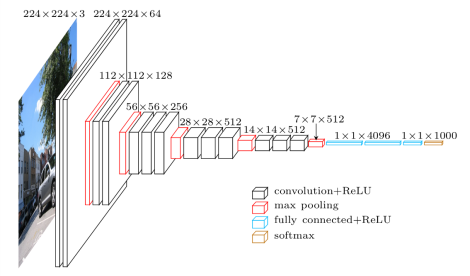
\includegraphics[width=\linewidth]{vgg16}
\caption{Schematic Diagram of VGG16 model}
\label{fig:vgg16schema}
\end{figure}
%
%VGG16 Model
%
%The script for fine--tuning VGG16 can be found in vgg16.py. 
%The first part of the vgg\_std16\_model function is the model schema for VGG16. 
%After defining the fully connected layer, we load the ImageNet pre--trained 
%weight to the model by the following line:

%model.load_weights('cache/vgg16_weights.h5')
%For fine-tuning purpose, we truncate the original softmax layer and replace it with our own by the following snippet:

%model.layers.pop()
%model.outputs = [model.layers[-1].output]
%%model.layers[-1].outbound_nodes = []
%model.add(Dense(num_class, activation='softmax'))
%Where the num\_class variable in the last line represents the number of class labels for our classification task.
%
%Sometimes, we want to freeze the weight for the first few layers so that they 
%remain intact throughout the fine-tuning process. 
%Say we want to freeze the weights for the first 10 layers. 
%%This can be done by the following lines:
%
%%for layer in model.layers[:10]:
%  %  layer.trainable = False
%We then fine-tune the model by minimizing the cross entropy loss function using
%stochastic gradient descent (sgd) algorithm. Notice that we use an initial learning 
%rate of 0.001, which is smaller than the learning rate for training scratch model 
%(usually 0.01).

%sgd = SGD(lr=1e-3, decay=1e-6, momentum=0.9, nesterov=True)
%model.compile(optimizer=sgd, loss='categorical_crossentropy', metrics=['accuracy'])
%model = vgg_std16_model(img_rows, img_cols, channel, num_class)
%Where img_rows, img_cols, and channel define the dimension of the input. For colored image with resolution 224x224, img_rows = img_cols = 224, channel = 3.

%Next, we load our dataset, split it into training and testing sets, and start fine-tuning the model:

%X_train, X_valid, Y_train, Y_valid = load_data()

%model.fit(train_data, test_data,
 %         batch_size=batch_size,
%          nb_epoch=nb_epoch,
 %         shuffle=True,
 %         verbose=1,
  %        validation_data=(X_valid, Y_valid),
 %         )
The fine-tuning process will take a while, depending on your hardware. 
After it is done, we use the model the make prediction on the validation set 
and return the score for the cross entropy loss:

%predictions_valid = model.predict(X_valid, batch_size=batch_size, verbose=1)
%score = log_loss(Y_valid, predictions_valid)


\subsection{Fine-tune Inception--V3}
\label{ssec:inception}
Inception--V3 achieved the second place in the $2015$ \emph{ImageNet} 
competition with a $5.6 \%$ top five error rate on the validation set. 
The model is characterized by the usage of the Inception Module, which is a 
concatenation of features maps generated by kernels of varying dimensions.
%
\begin{figure}[htb]
\centering
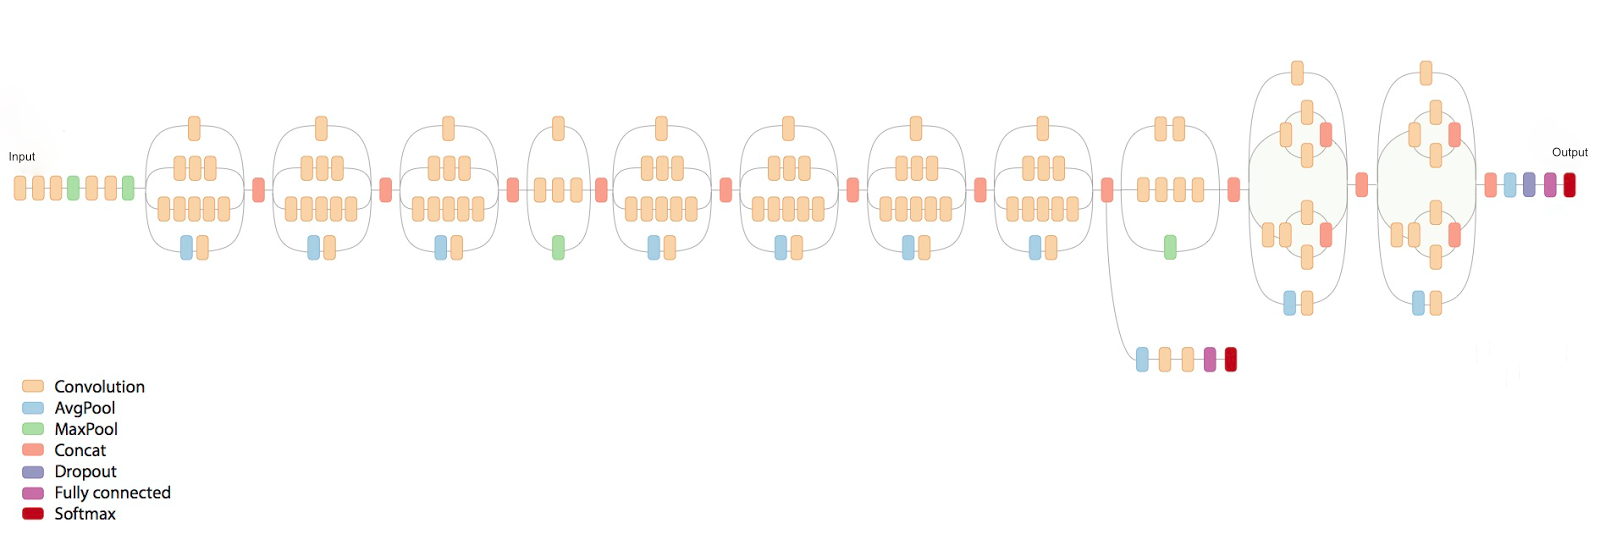
\includegraphics[width=\linewidth]{inception}
\caption{Schematic Diagram of Inception--V3 model}
\label{fig:inceptionV3schema}
\end{figure}
%
